\documentclass[main.tex]{subfiles}


% Cowan_2011
\begin{document}

\section{Overview}

This analysis utilizes a binned liklihood-maximization technique comparing some observation, whether it is true data or pseudo-data, against Monte Carlo simulation weighted to the expectation from multiple sterile neutrino hypothesis. 
Binning is done on reconstructed quantities; bins are linearly spaced in $\cos\theta_{reco}$ and logarithmically spaced in $E_{reco}$. 
Sterile neutrino points are chosen uniformly over $\left|U_{\mu 4}\right|^{2}=\sin^{2}\theta_{24}$, $\left|U_{\tau 4}\right|^{2}=\sin^{2}\theta_{34}\cos^{2}\theta_{24}$, and $\Delta m_{41}^{2}$. 
A 16 by 16 grid in the unitary mixing matrix elements, and five discrete mass-squared splittings are explored. 
These five values are 
\begin{enumerate}
    \item 1.0eV$^{2}$ - a commonly chosen value used in sterile oscillations studies. 
    \item 3.5eV$^{2}$ - a value close to the best-fit point from BEST~\cite{barinov2021results}
    \item 4.5eV$^{2}$ - a value close to the eight-year IceCube through-going track analysis~\cite{Aartsen_2020, Aartsen_2020_prd}
    \item 10.0eV$^{2}$ - an intermediate value between those above, and larger mass-squared splitting
    \item 100.0eV$^{2}$ - a larger mass-squared splitting where fast oscillations will dominate the signal. 
\end{enumerate}



\section{Cascade Event Selection}

\subsection{Topological Splitting}

Before further processing and reconstruction is done on events, filter is applied to reduce the cosmic ray muon background while maintaining atmospheric signals as efficiently as possible. 
The first step of this process implements a topological triggering which distinguishes events between coincident and non-coincident events; the later of which are discarded. 
After this, events are classified as either contained within the detector or ``through going." For the cascades sample only those events contained within the detector are considered. 

Contained events must satisfy several criteria:
\begin{itemize}
    \item The depth of the first detected light must be greater than 70 meters from the outer edge of IceCube
    \item The first detected light must not be the outer layer of IceCube
\end{itemize}

\begin{enumerate}
    \item The number of topological splits must be one; coincident events are discarded
    \item The event must be contained 
\end{enumerate}

\subsection{Final Level Filtering}

This final level event filter was developed and published in Ref~\cite{2018PhDT17N}.

The monopod reconstruction algorithm is then run on events which survive the topological splitting cuts. 
This algorithm, in addition to calculating a reconstructed energy, interaction vertex, and direction, calculates a  reduced likelihood for the fit; the smaller the reduced log-likelihood is the better. 
Events for which the reduced algorithm fail, or are poor quality, are discarded. 
A poor quality reconstruction is one with a reduced log-likelihood of greater than 9.1.
Events within the IceCube dust-layer must have either 

Strict containment based on the reconstruction of the vertex coordinates from Monopod. 

Tighter coordinates cut at the top and bottom of the detector. For those just outside an inner, fiducial, volume, we keep events only if they are well-reconstructed with a reduced log-likelihood<7.5. 

Finally, we cut those events with very large, negative, photon delay times. Such large delay times are common for detector triggers resulting from uncorrelated bundles of atmospheric cosmic ray muons. 

\section{Track Event Selection}

The track sample of this analysis uses events with reconstructed energies between 500GeV and 10 TeV. 
The event selection is constructed from a series of cuts, described briefly here, and at length in References~\cite{Aartsen_2020, Aartsen_2020_prd, axani2020sterile}. % 50, 68, 69, 129

\begin{enumerate}
    \item Discard events for which fewer than fifteen DOMs are triggered or fewer than six are triggered on direct light.
    \item  For events with $0\leq\cos\theta_{\mu}^{reco}\leq 0.2$, discard if the total charge $Q_{tot}<100$ photoelectrons (PEs) or if the average weighted charge distance $<200$ meters/PE. 
    \item Remove all events with a reconstructed value of $\cos\theta_{\mu}^{reco}\geq 0.2$. This removes down-going track like events that are likely cosmic ray muons. 
    \item Discard all events with a reconstructed track length less than 200 meters, or a track smoothness $<0.6$.
\end{enumerate}

These cuts comprise the ``Golden Filter,'' described in Ref REF, and produce a sample with $\nu_{\mu}$ purity greater than 99\%. %129
An additional, ``Diamond filter,'' is used to further improve sample quality. 
It uses an additional set of cuts
\begin{enumerate}
    \item Discard events with fewer than twelve direct light DOM triggers. 
    \item Discard events with $Q_{tot}\leq20$ PE outside DeepCore. 
    \item Discard events with fifteen or fewer DOMs triggered outside DeepCore. 
    \item Discard events with $\cos\theta_{\mu}^{reco}>0.05$.
\end{enumerate}

\section{Likelihood Metric}\label{sect:llh_metric}

The likelihood used in this analysis is defined as the probability of observing a given set of data, or pseudo-data, assuming some physics hypothesis.
It is quantified as 
\begin{equation}
    \mathcal{L}(\vec{\Theta}, \vec{\eta}) = \prod_{i=0}^{\text{bins}} \mathcal{L}_{eff}\left( w_{i}^{sum}, w_{2,i}^{sum}, k_{i} \right),
\end{equation}
where $w_{i}$ and $w_{2,i}$ are the sums of the MC weights and MC weights squared, respectively, in bin $i$; $k_{i}$ is the observed number of events (or pseudo-events). 
$\vec{\Theta}$ is the tested physics hypothesis and $\vec{\eta}$ the set of nuisance parameters. 

The effective likelihood function, defined in Ref~\cite{effective_llh}, is part of a family of likelihood metrics used to account for MC statistical uncertainty. 
We use the form where
\begin{align}
    \alpha&=\dfrac{\mu^{2}}{\sigma^{2}} +1 & &\text{and} & \beta&=\dfrac{\mu}{\sigma^{2}}.
\end{align}
Since each simulated MC event is just one event, $\mu = w_{i}$ and $\sigma^{2} = w_{2,i}$\footnote{it is possible to merge MC events into `meta-events' to speed up reweighting, where the functional forms are slightly more complicated. This, however, is not done in this analysis}, and
\begin{equation}
    \mathcal{L}_{eff}(\vec{\Theta} | k) = \left(\dfrac{\mu}{\sigma^{2}}\right)^{\tfrac{\mu^{2}}{\sigma^{2}} + 1} \Gamma\left(k + \dfrac{\mu^{2}}{\sigma^{2}} + 1\right) \left[ k! \left(1+\dfrac{\mu}{\sigma^{2}}\right)^{k+\tfrac{\mu^{2}}{\sigma^{2}} + 1} \Gamma\left(\dfrac{\mu^{2}}{\sigma^{2}} +1\right)\right]^{-1}
\end{equation}
where $\Gamma$ is the gamma function. 

The set of nuisance parameters describe that describe systematic uncertainties are themselves constrained by Gaussian priors functions. 
These priors are used to weight the likelihoods, which is maximized to form a profile likelihood, defined as 

\begin{equation}
\mathcal{L}_{\text{profile}}\left(\vec{\theta}\right) = \text{max}_{\vec{\eta}}\left[\mathcal{L}(\vec{\Theta}, \vec{\eta}) \Xi(\vec{\eta}) \right]
\end{equation}
where $\Xi(\vec{\eta})$ is the total likelihood penalty for the set of nuisance parameters $\vec{\eta}$ calculated accounting for the correlations between the priors. 

We then construct an analysis test statistic (TS) for producing confidence intervals, which we define as 
\begin{equation}\begin{split}
TS(\vec{\Theta}) &= -2\left[ \log\mathcal{L}_{\text{profile}}(\vec{\theta}) - \log\mathcal{L}_{\text{profile}}(\vec{\Theta}_{min}) \right] \\
&= -2 \Delta \log\mathcal{L}_{\text{profile}}(\vec{\theta})\\
&=-2\Delta \text{LLH}
\end{split}\end{equation}
where $\vec{\Theta}_{min}$ is the sterile hypothesis that maximizes the likelihood, and best matches the data: the best fit point. 

\textit{Short discussion about biases introduced by this likelihood function}

\section{Tests}

A series of tests were performed to validate the implementation of the nuisance parameters and verify the performance of the fitting framework. 

\subsection{Inject-Recover Systematic Tests}

Pseudo-experimental results, or `realizations,' are first calculated by perturbing each nuisance parameter some amount, individually, and getting the expected event rates without additional statistical variation applied. 
This is done for each nuisance parameter allowed to float in the fit, for amounts across the whole range given by the parameters' priors. 
Fits are then carried out to each of these realizations.

The results are tabulated below in two figures: in Figure~\ref{fig:ir_nopriorpert} the results are shown where the prior on the nuisance parameter is left at its original value; in Figure~\ref{fig:ir_priorpert} the prior is changed to the value of the injected nuisance parameter. 
For the most part, in Figure~\ref{fig:ir_priorpert}, the exact value injected is recovered by the fitter. 
In a few cases, notably for the \texttt{aeff\_scale} and \texttt{astro\_norm\_rotated} parameters, there are misfits when the injected parameter pulls near the edge of the range of the parameter.
Given this only happens for large deviation, it is not of concern. 
Another feature of note occurs for
The parameters show a systematic deviation that increases as the injected parameter is further from the nominal value. 
The parameter most strongly exhibiting this effect is \texttt{vhe3\_piplus\_rot}, where at high, positive, perturbation the fit value is systematically lower; the converse is true for a negative perturbation. 
This effect appears consistent with a minor bias that can be introduced by the effective likelihood function\footnote{See the discussion in Section~\ref{sect:llh_metric}} in cases of large MC statistical error.  

In Figure~\ref{fig:ir_nopriorpert}, the flatter a parameter is then the more tightly-constrained its prior is. 

\begin{figure}
    \centering 
    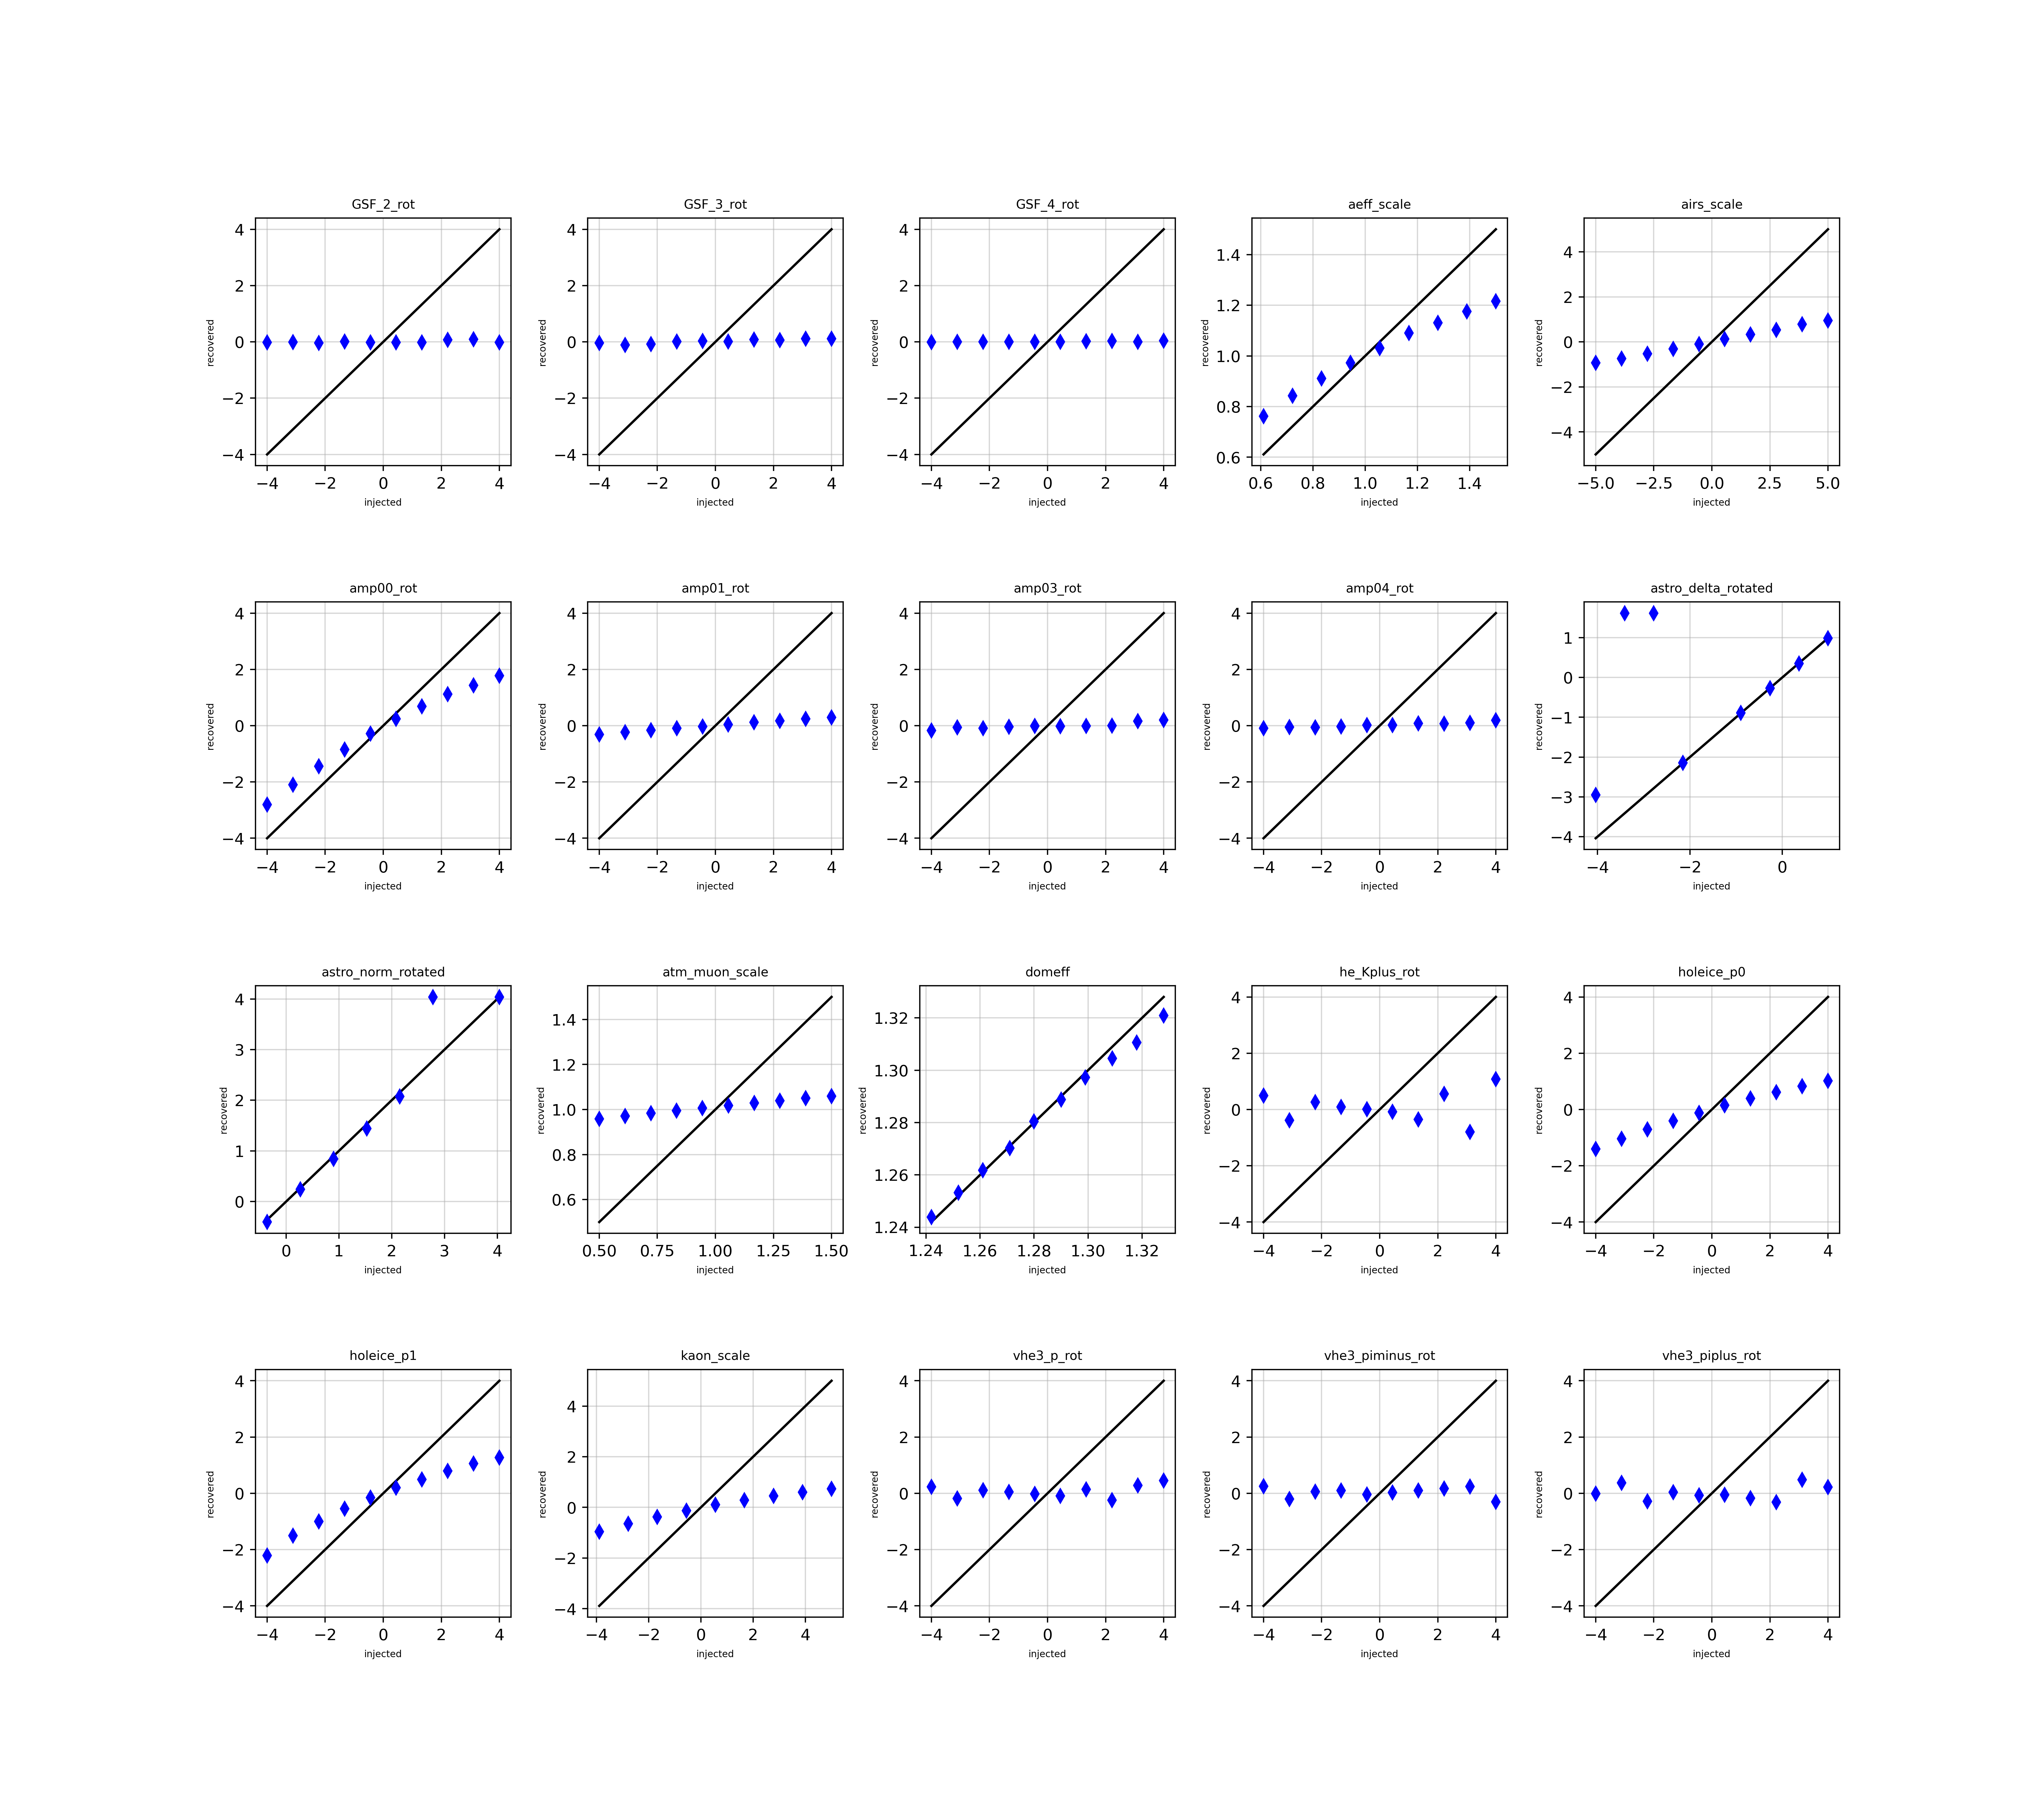
\includegraphics[width=0.7\linewidth]{figures/inject_recover_syst.png}
    \caption{Fit results after injecting various perturbed values for each nuisance parameter and running the fitter. }\label{fig:ir_nopriorpert}
\end{figure}


\begin{figure}
    \centering 
    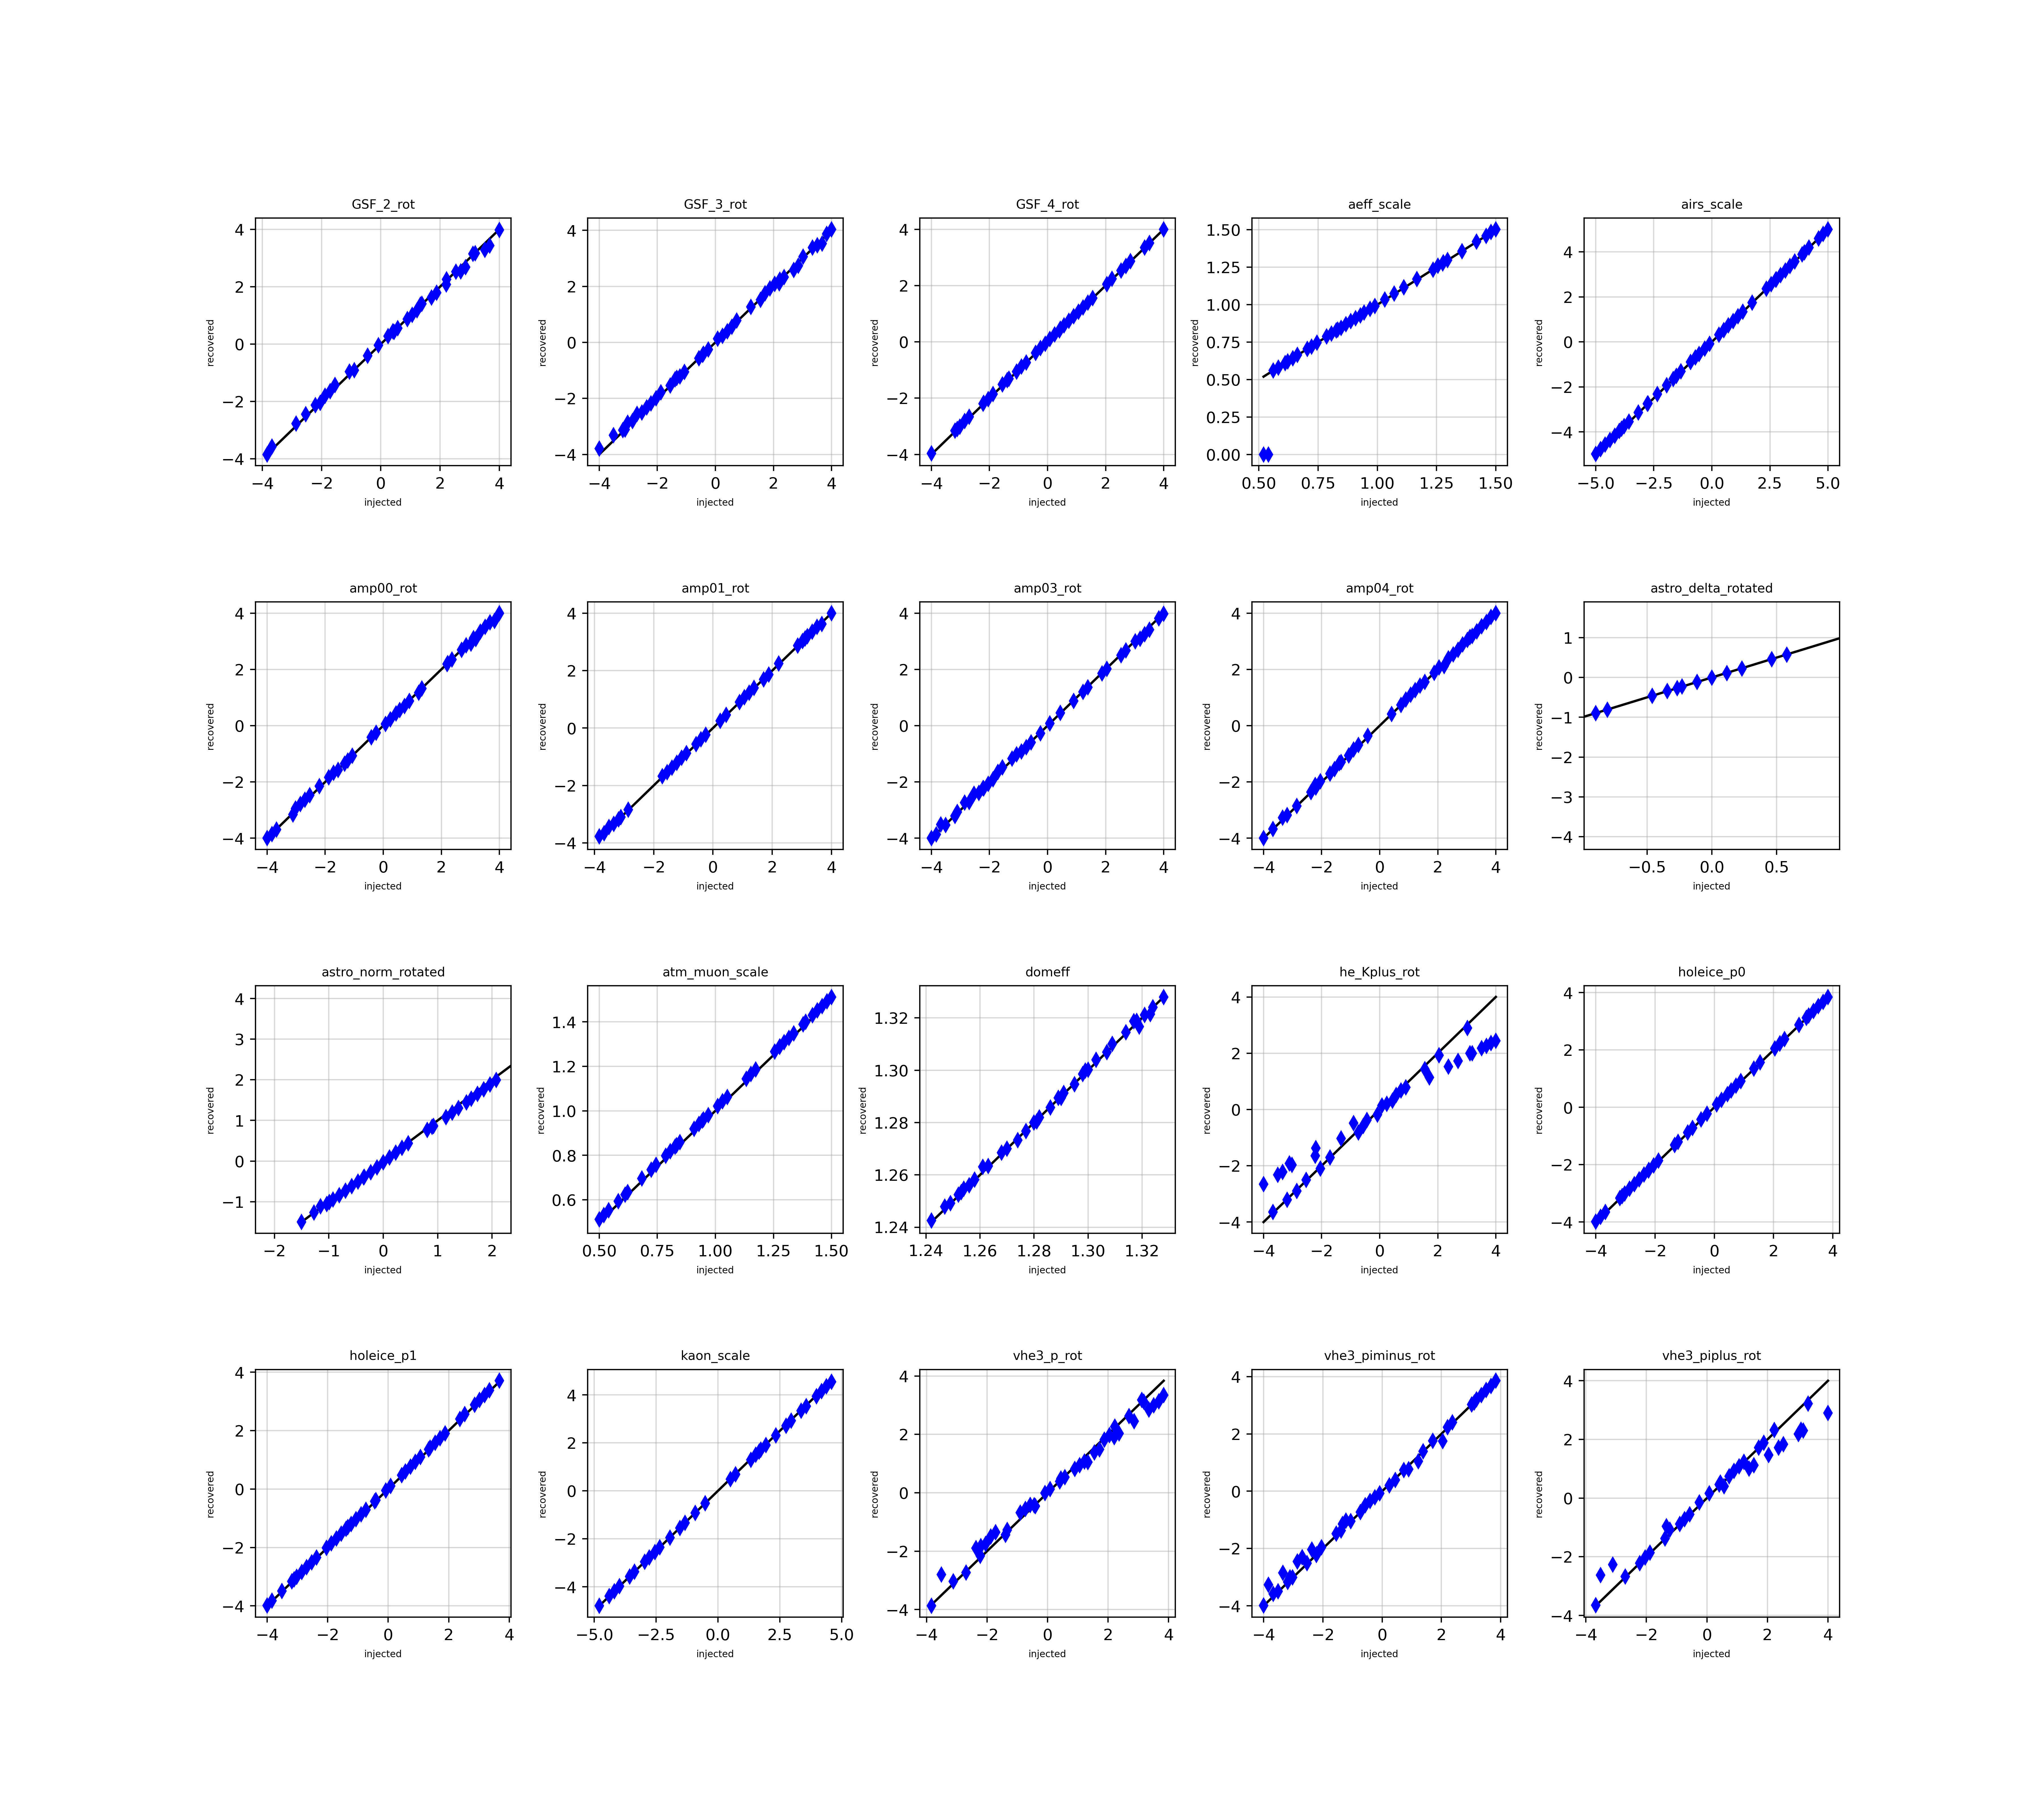
\includegraphics[width=0.7\linewidth]{figures/inject_recover_syst_prior.png}
    \caption{Fit results after injecting various perturbed values for each nuisance parameter and running the fitter. Priors are adjusted in each fit according to the injected values.}\label{fig:ir_priorpert}
\end{figure}

\subsection{Asimov Sensitivity}

First, a single realization was generated without applying statistical variation on the per-bin expectation. 
This is the Asimov realization. 
Fits were performed for this simulated observation and test scores were calculated for each one following the metrics defined in Section~\ref{sect:llh_metric}.
The 90\% confidence level $\chi^{2}$ threshold was calculated for three degrees of freedom for the fit scan, and the resulting sensitivity contours are shown in Figure~\ref{fig:asimov_sense}. 
These results are plotted, superimposed against other experiment's sensitivities, in Figure~\ref{fig:asimov_compare}. 
Sensitivities are compared at 90\% confidence level and assuming two degrees of freedom $\Delta m_{41}^{2}=$ 1.0 eV$^{2}$, where unfortunately sensitivity for this analysis has been observed to be at its worst. 
To provide a similar comparison, we also include the 90\% confidence level sensitivity contours with two degrees of freedom at $\Delta m_{41}^{2}=$ 4.5 eV$^{2}$ as well in the right panel of Figure~\ref{fig:asimov_compare}.

The sensitivities here are observed to be worse than those predicted earlier in Chapter~\ref{chapter:sense}, though this is not surprising. 
Previous predictions used very approximate representation of the nuisance parameters present in IceCube. 
In addition to this, the muon background was not included in the previous sensitivity calculations.

\begin{figure}
    \centering
    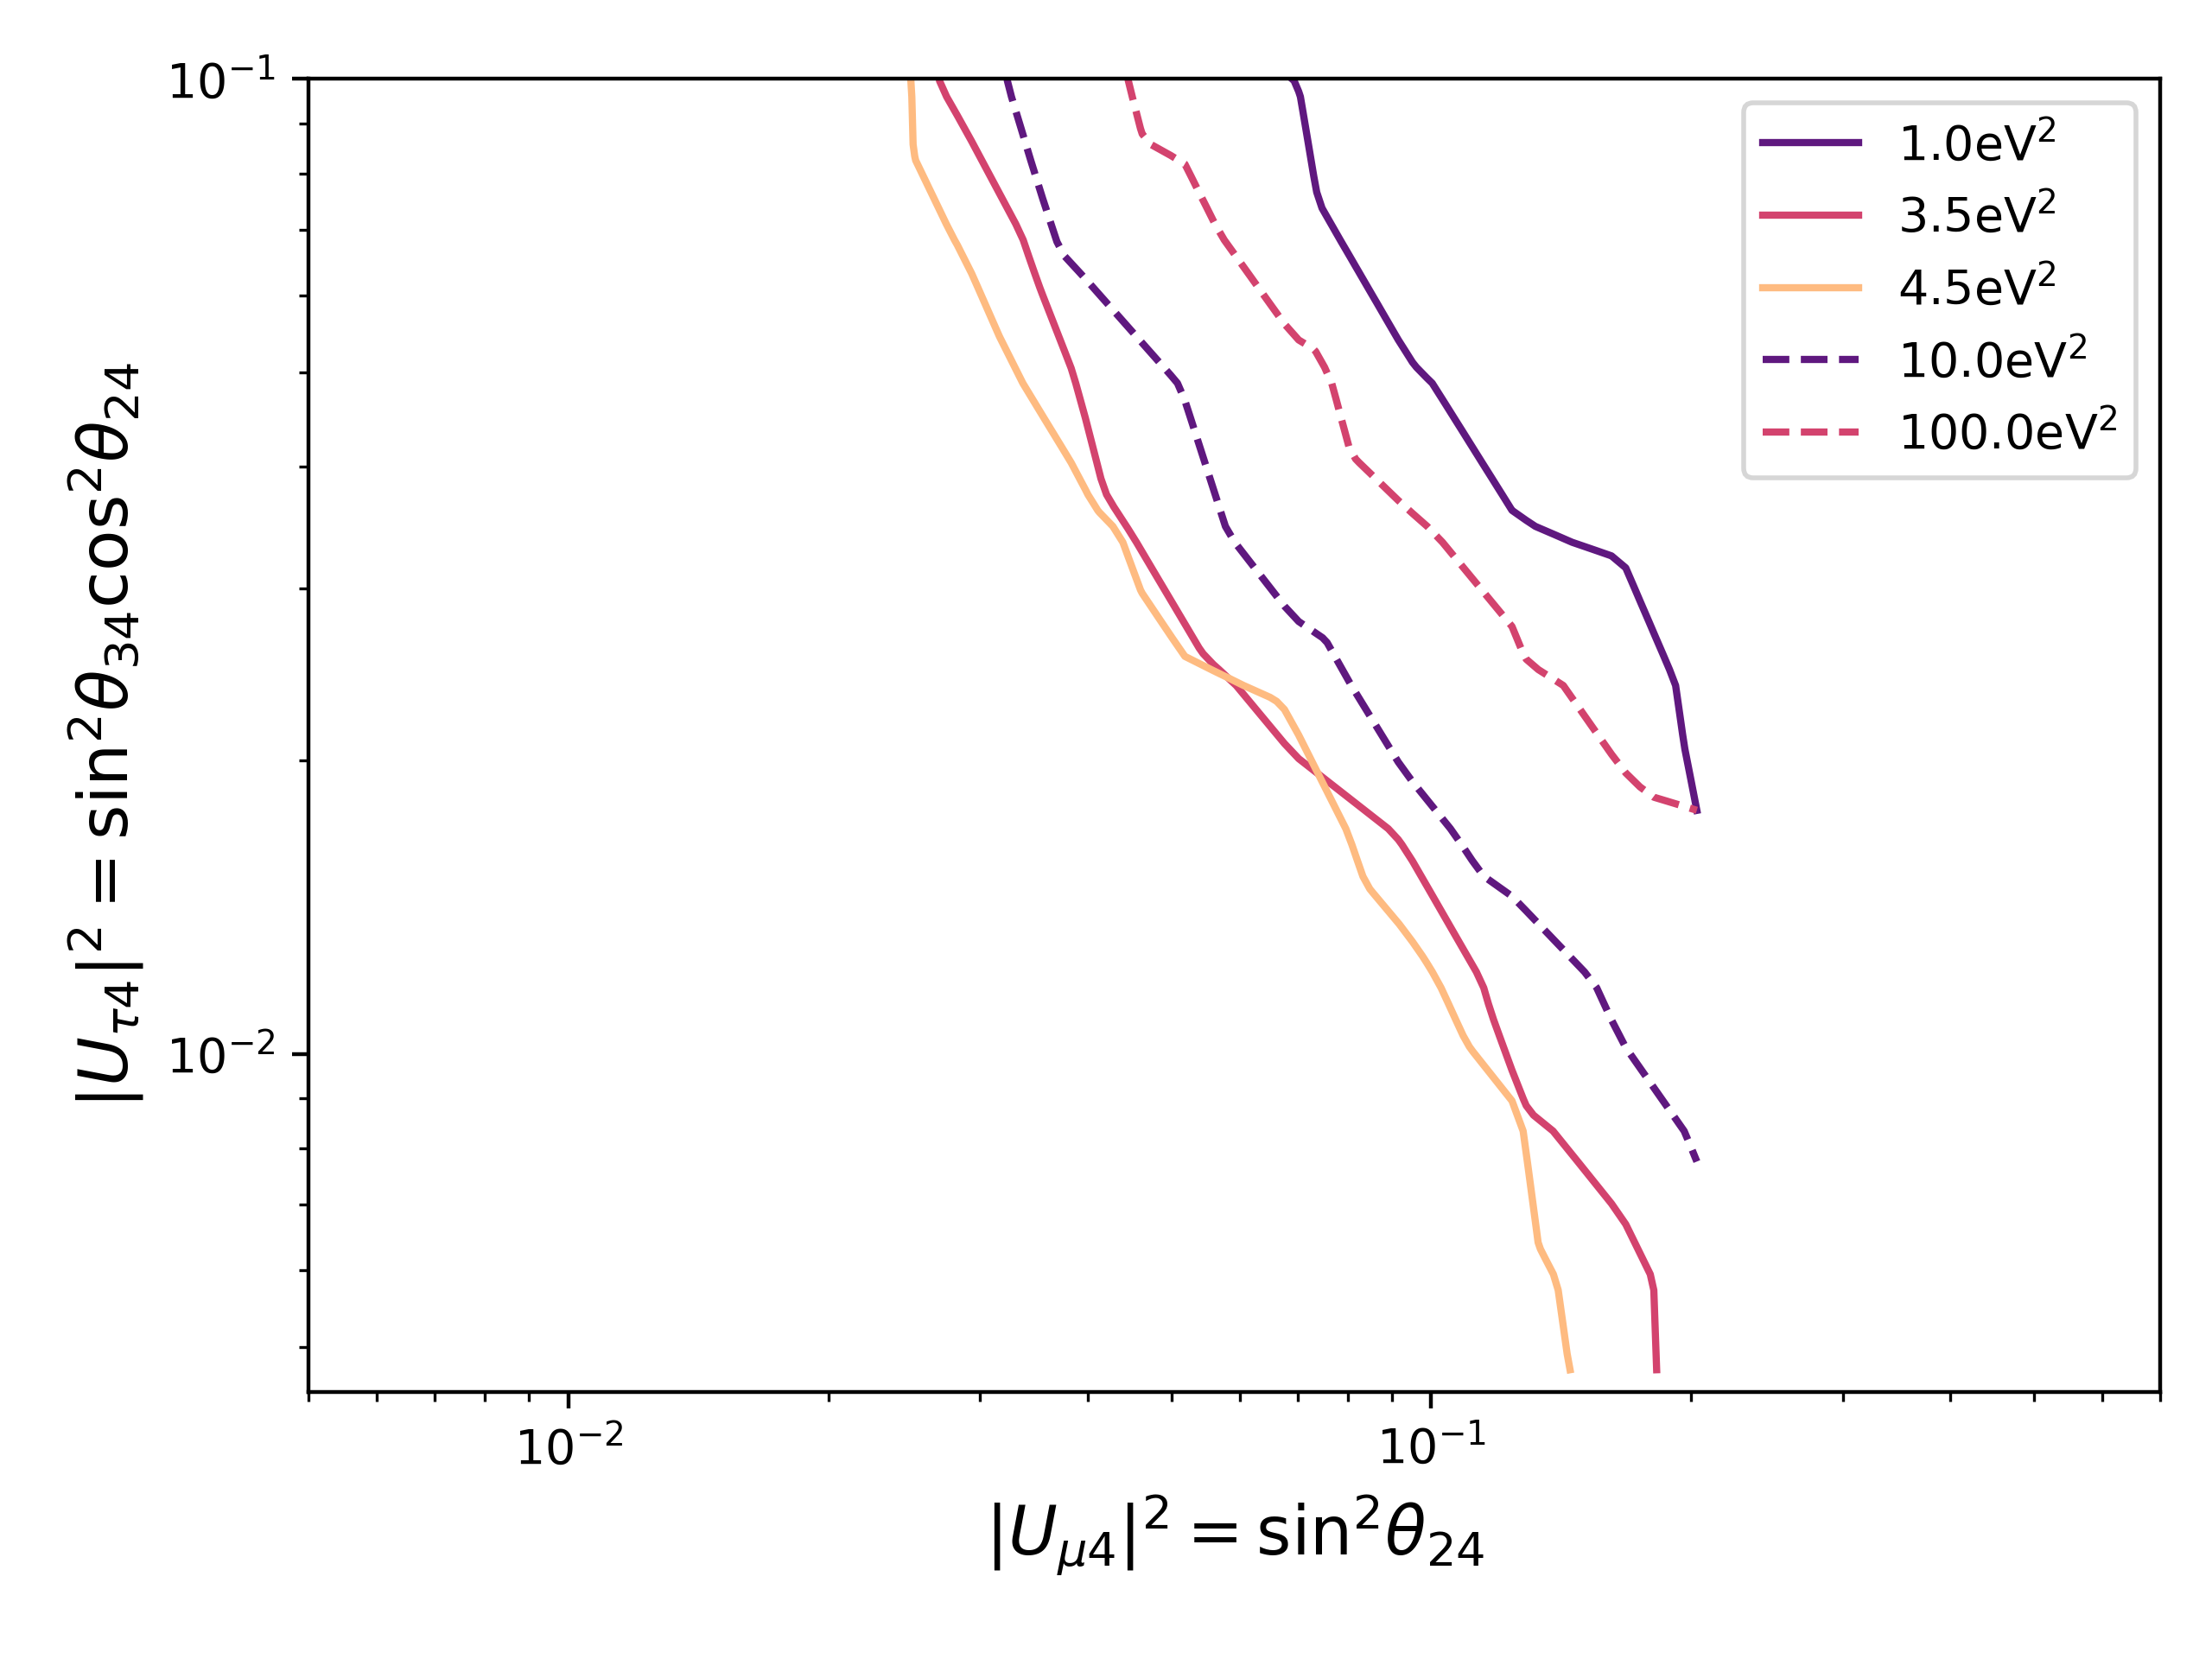
\includegraphics[width=0.7\linewidth]{figures/cascade_mcllheff_final_Realization_Asimov_sterile_0_cl0.9_dof3.png}
    \caption{The 90\% confidence level sensitivity contours with three degrees of freedom for this analysis.}\label{fig:asimov_sense}
\end{figure}

\begin{figure}
    \centering
    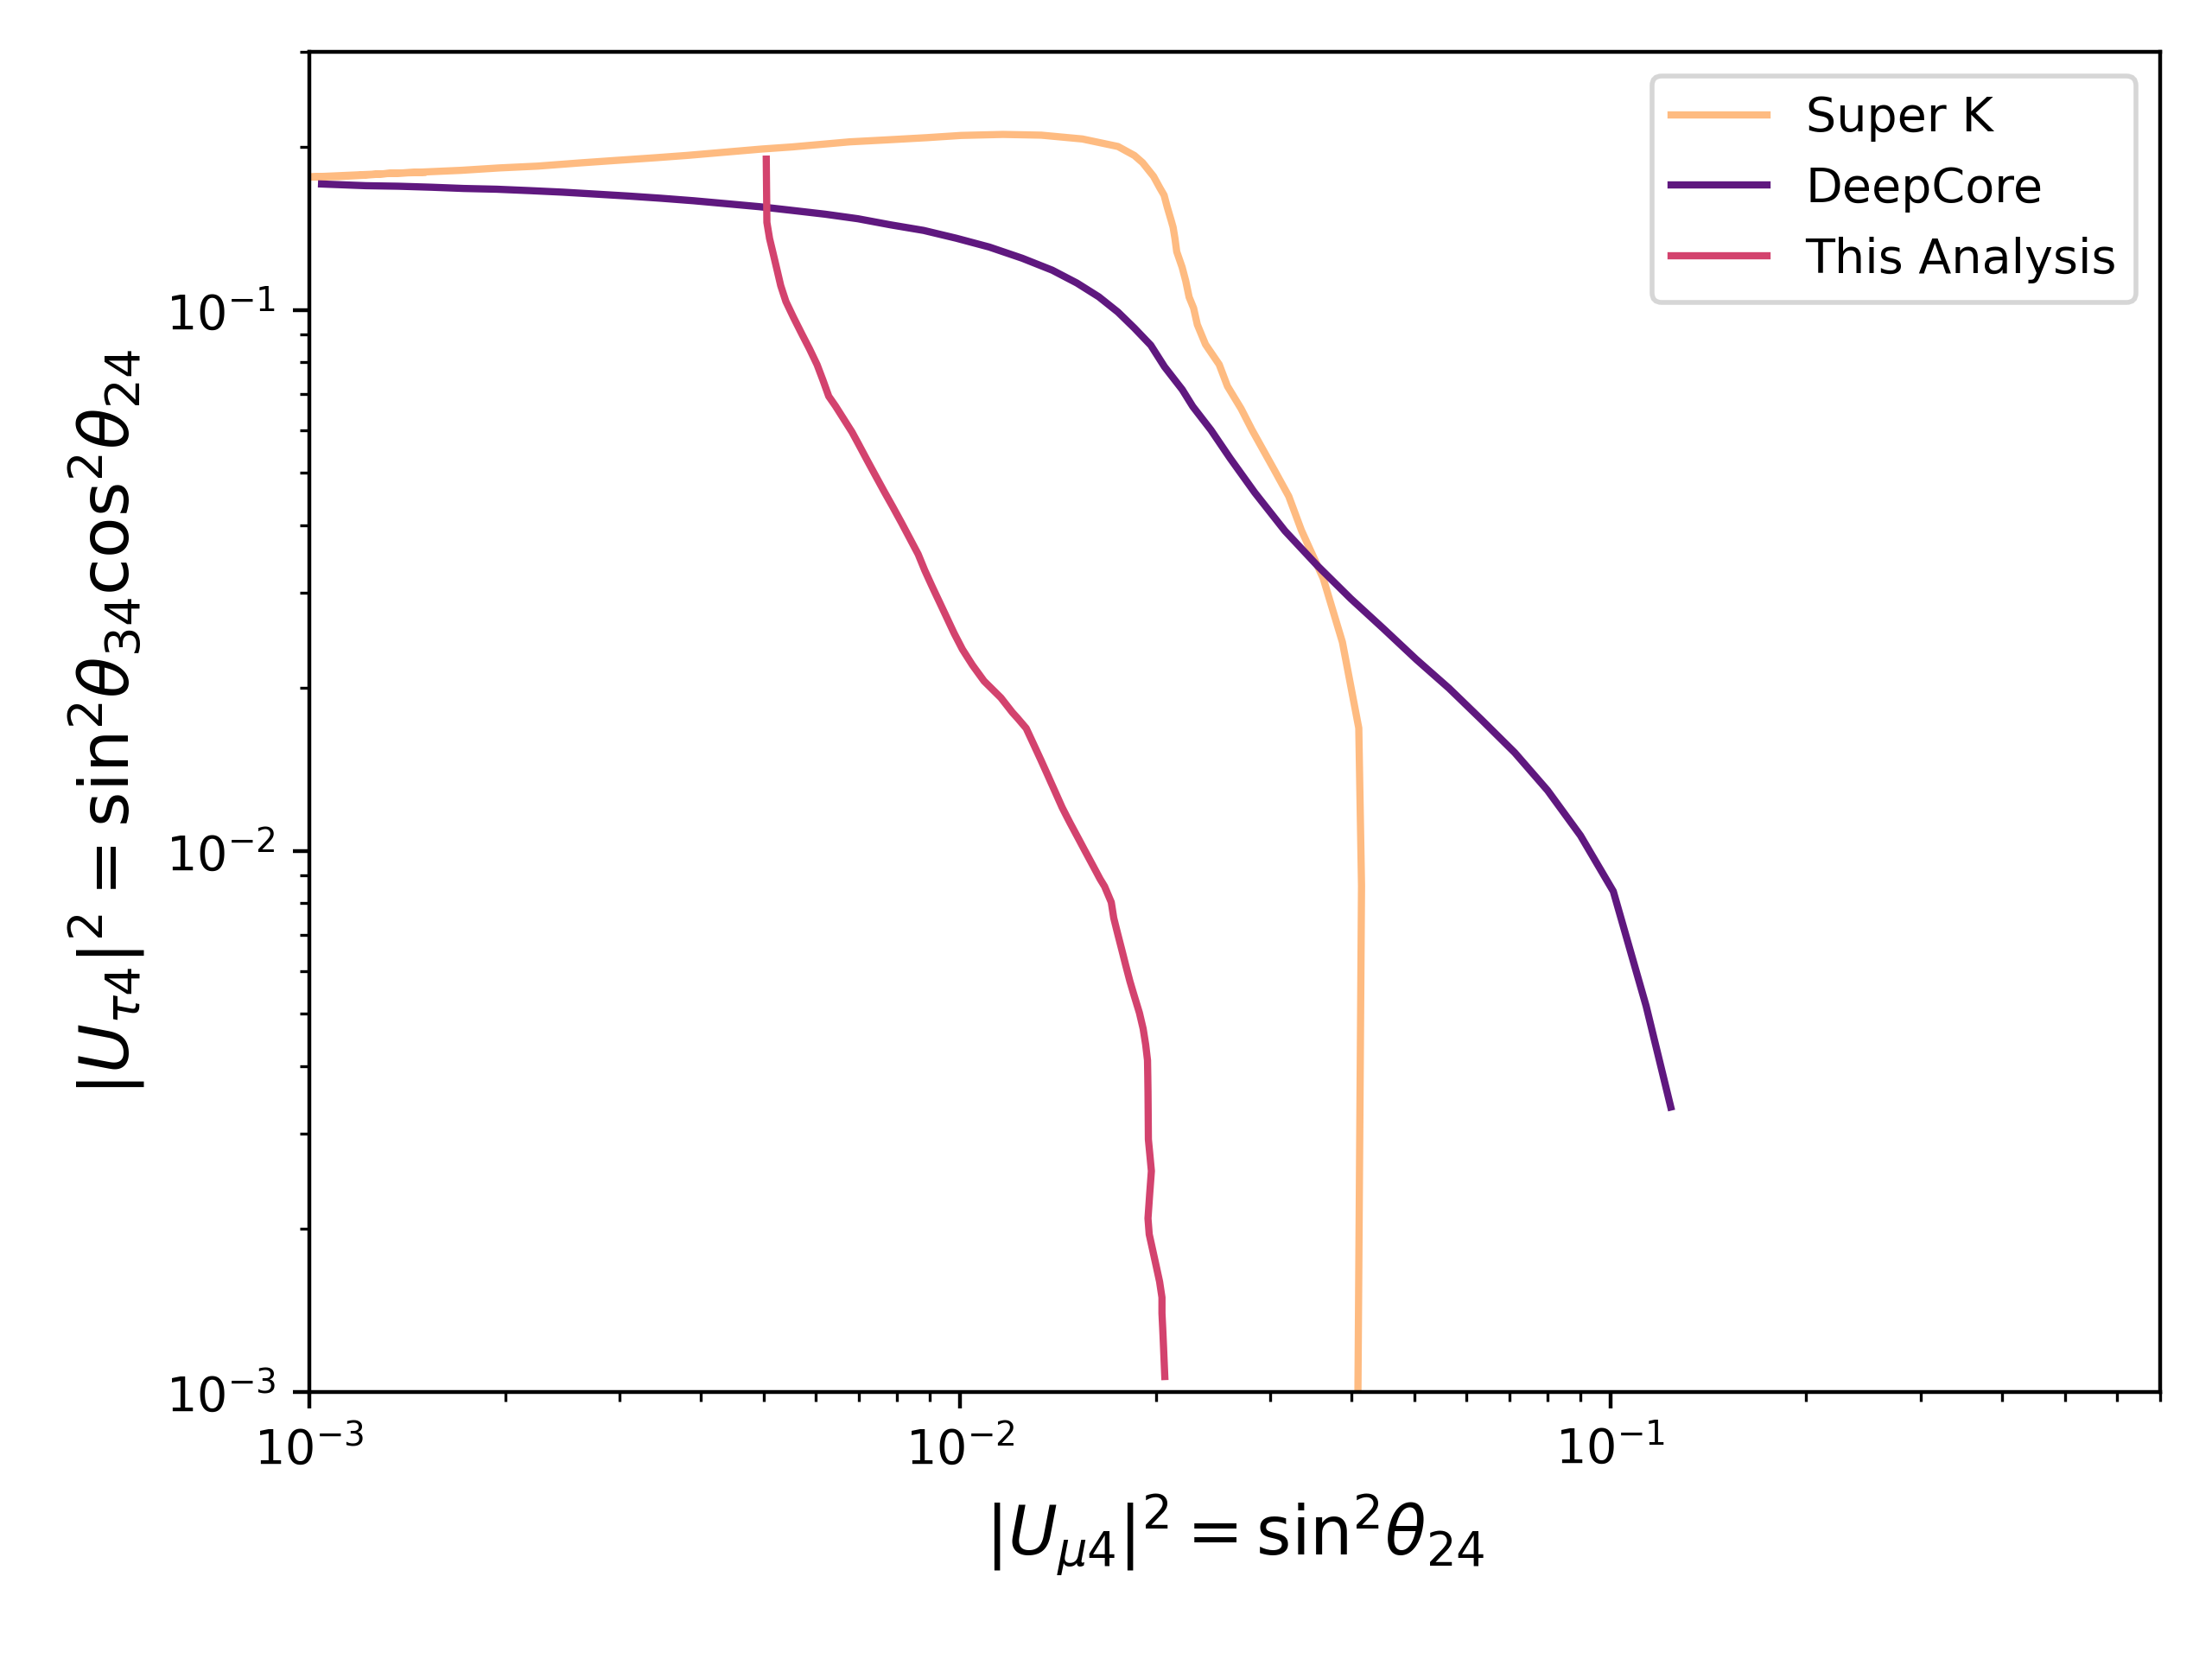
\includegraphics[width=0.45\linewidth]{figures/comparison.png}%
    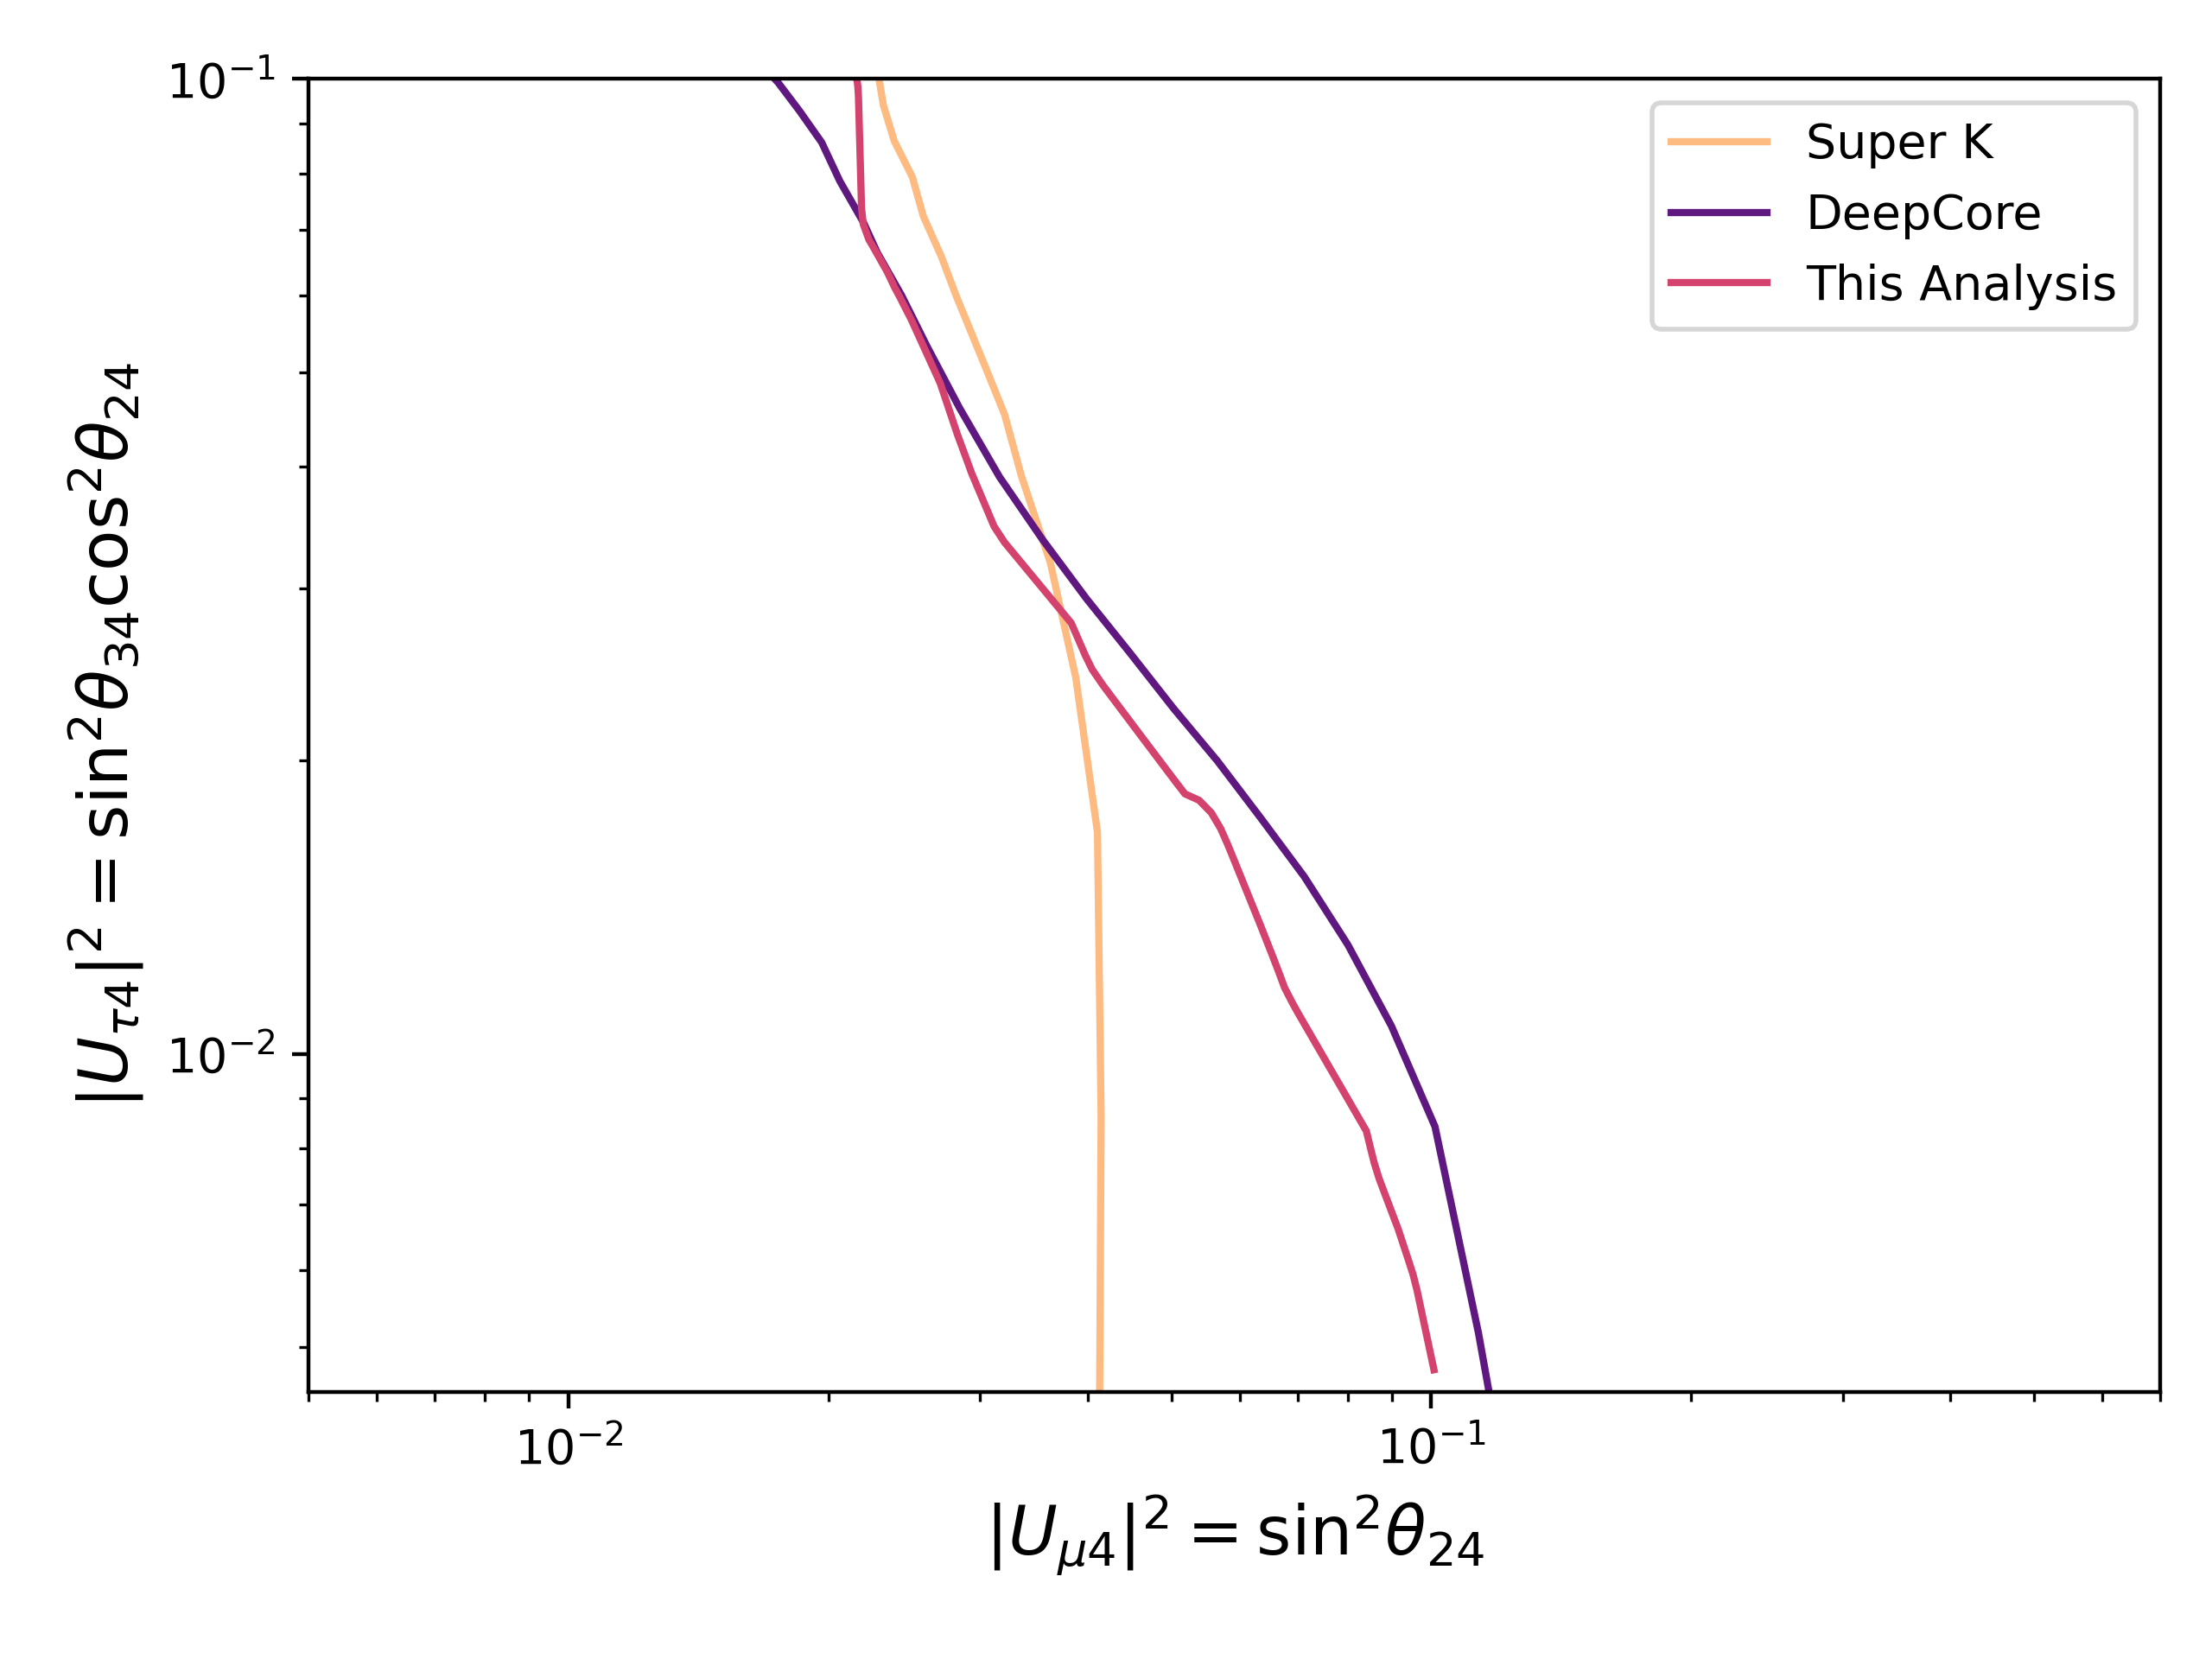
\includegraphics[width=0.45\linewidth]{figures/comparison_45.png}%
    \caption{The 90\% confidence level sensitivity contours for this analysis with two degrees of freedom at $\Delta m_{41}^{2}=$ 1.0 eV$^{2}$ (left), and  4.5 eV$^{2}$ (right), are shown. Senstivities from DeepCore~\cite{Aartsen_2017_dc} and Super-K~\cite{PhysRevD.91.052019} at 1.0eV$^{2}$ are also shown.}\label{fig:asimov_compare}
\end{figure}



\subsection{Systematic Impact Tests}

Nuisance parameters were collected into ``bundles.'' 
Asimov sensitivity scans~\cite{Cowan_2011} were then performed for each bundle while fixing the parameters of that bundle to their central values.
The resulting confidence intervals then show the impact of fixing those nuisance parameters. 
The bundles are 
\begin{enumerate}
    \item Conv(entional): Daemonflux~\cite{yanez2023daemonflux} parameters, AIRS scale, and the kaon-nucleon cross section uncertainty
    \item Astr: astrophysical normalization and the spectral index
    \item Det(ector): hole ice uncertainty, DOM efficiency, and the bulk-ice uncertainty
    \item Muon: the CR muon background\footnote{Because of the large, extra, error introduced by the muon background, for this systematic impact test a special realization is generated and fit to where there no muon contribution is added at all.}
    \item Normalization (aeff\_scale): overall normalization
\end{enumerate}
These sensitivity contours are shown at 90\% confidence level and with three degrees of freedom in Figure~\ref{fig:impact}

\begin{figure}
    \centering
    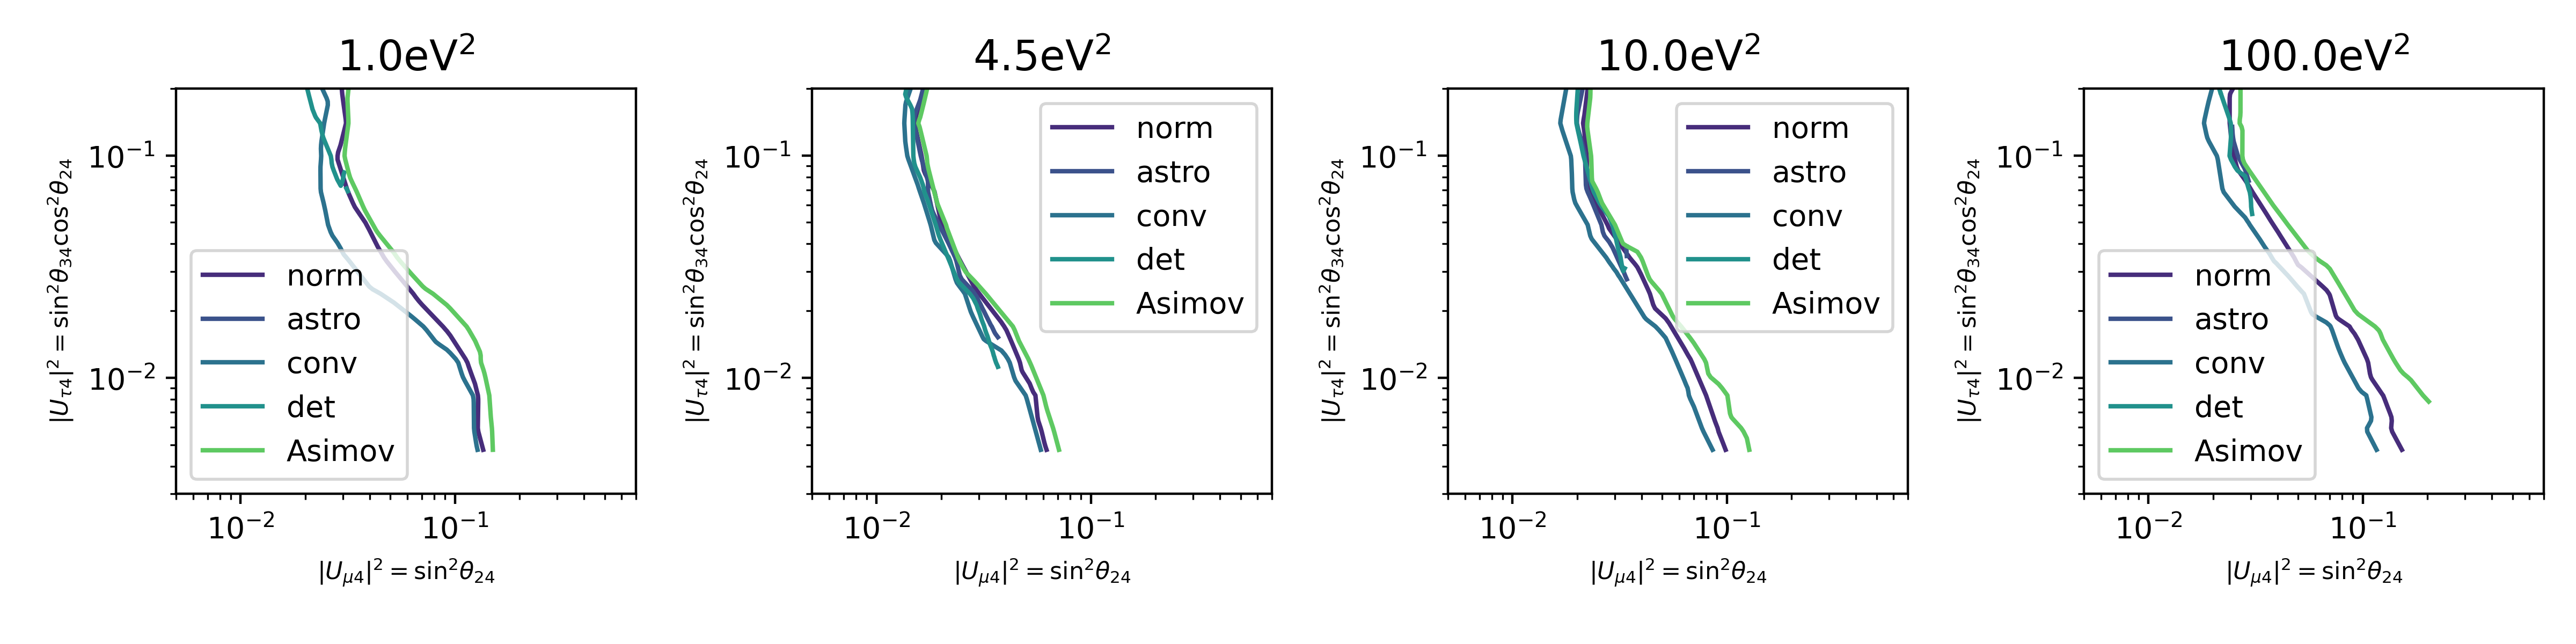
\includegraphics[width=0.90\linewidth]{figures/systematic_impact.png}
    \caption{The sensitivity contours for fixing each bundle of nuisance parameters. Contours are shown at 90\% CL and 3DOF for various mass-squared splittings; from left to right: 1.0eV$^{2}$, 4.5eV$^{2}$, 10.0eV$^{2}$, and 100.0eV$^{2}$.}\label{fig:impact}
\end{figure}

\subsection{Signal Inject-Recover}

Various points were chosen along the Asimov 90\% CL thresholds to test the fitters ability to recover constraints of sterile-neutrino signal-like measurements. 
Two each were chosen along the contours at 1.0, 4.5, 10, and 100 eV$^{2}$. 
Additionally, one more point was chosen off-grid. 
Each of these points are listed in Table~\ref{table:injected_signals}.

\begin{table}
    \centering
    \rowcolors{2}{gray!25}{white}
    \begin{tabular}{c | cccc}\rowcolor{blue!25}
            Realization Name & $\theta_{14}$ & $\theta_{24}$ & $\theta_{34}$ & $\Delta m_{41}^{2}$ [eV$^{2}$] \\
            RealIR\_0 & 0.0 & 0.492 & 0.104 & 1.0 \\
            RealIR\_1 & 0.0 & 0.685 & 0.505 & 1.0 \\
            RealIR\_2 & 0.0 & 0.310 & 0.234 & 4.5 \\
            RealIR\_3 & 0.0 & 0.171 & 0.324 & 4.5 \\
            RealIR\_4 & 0.0 & 0.147 & 0.110 & 10.0 \\
            RealIR\_5 & 0.0 & 0.171 & 0.324 & 10.0 \\
            RealIR\_6 & 0.0 & 0.147 & 0.132 & 100 
    \end{tabular}
    \caption{Sterile neutrino mixing angles at which Asimov realizations were generated.}\label{table:injected_signals}
\end{table}

Then, we ran a full fit-scan on an Asimov realization generated for each of these simulated signals. 
The contours are shown in the Figure FIG. 


\textit{Discussion of the constraints}

\end{document}